\section{Appendix}\label{sec:appendix}
TODO hyperparameters, tables

\begin{figure}[!tbp]
  \centering
  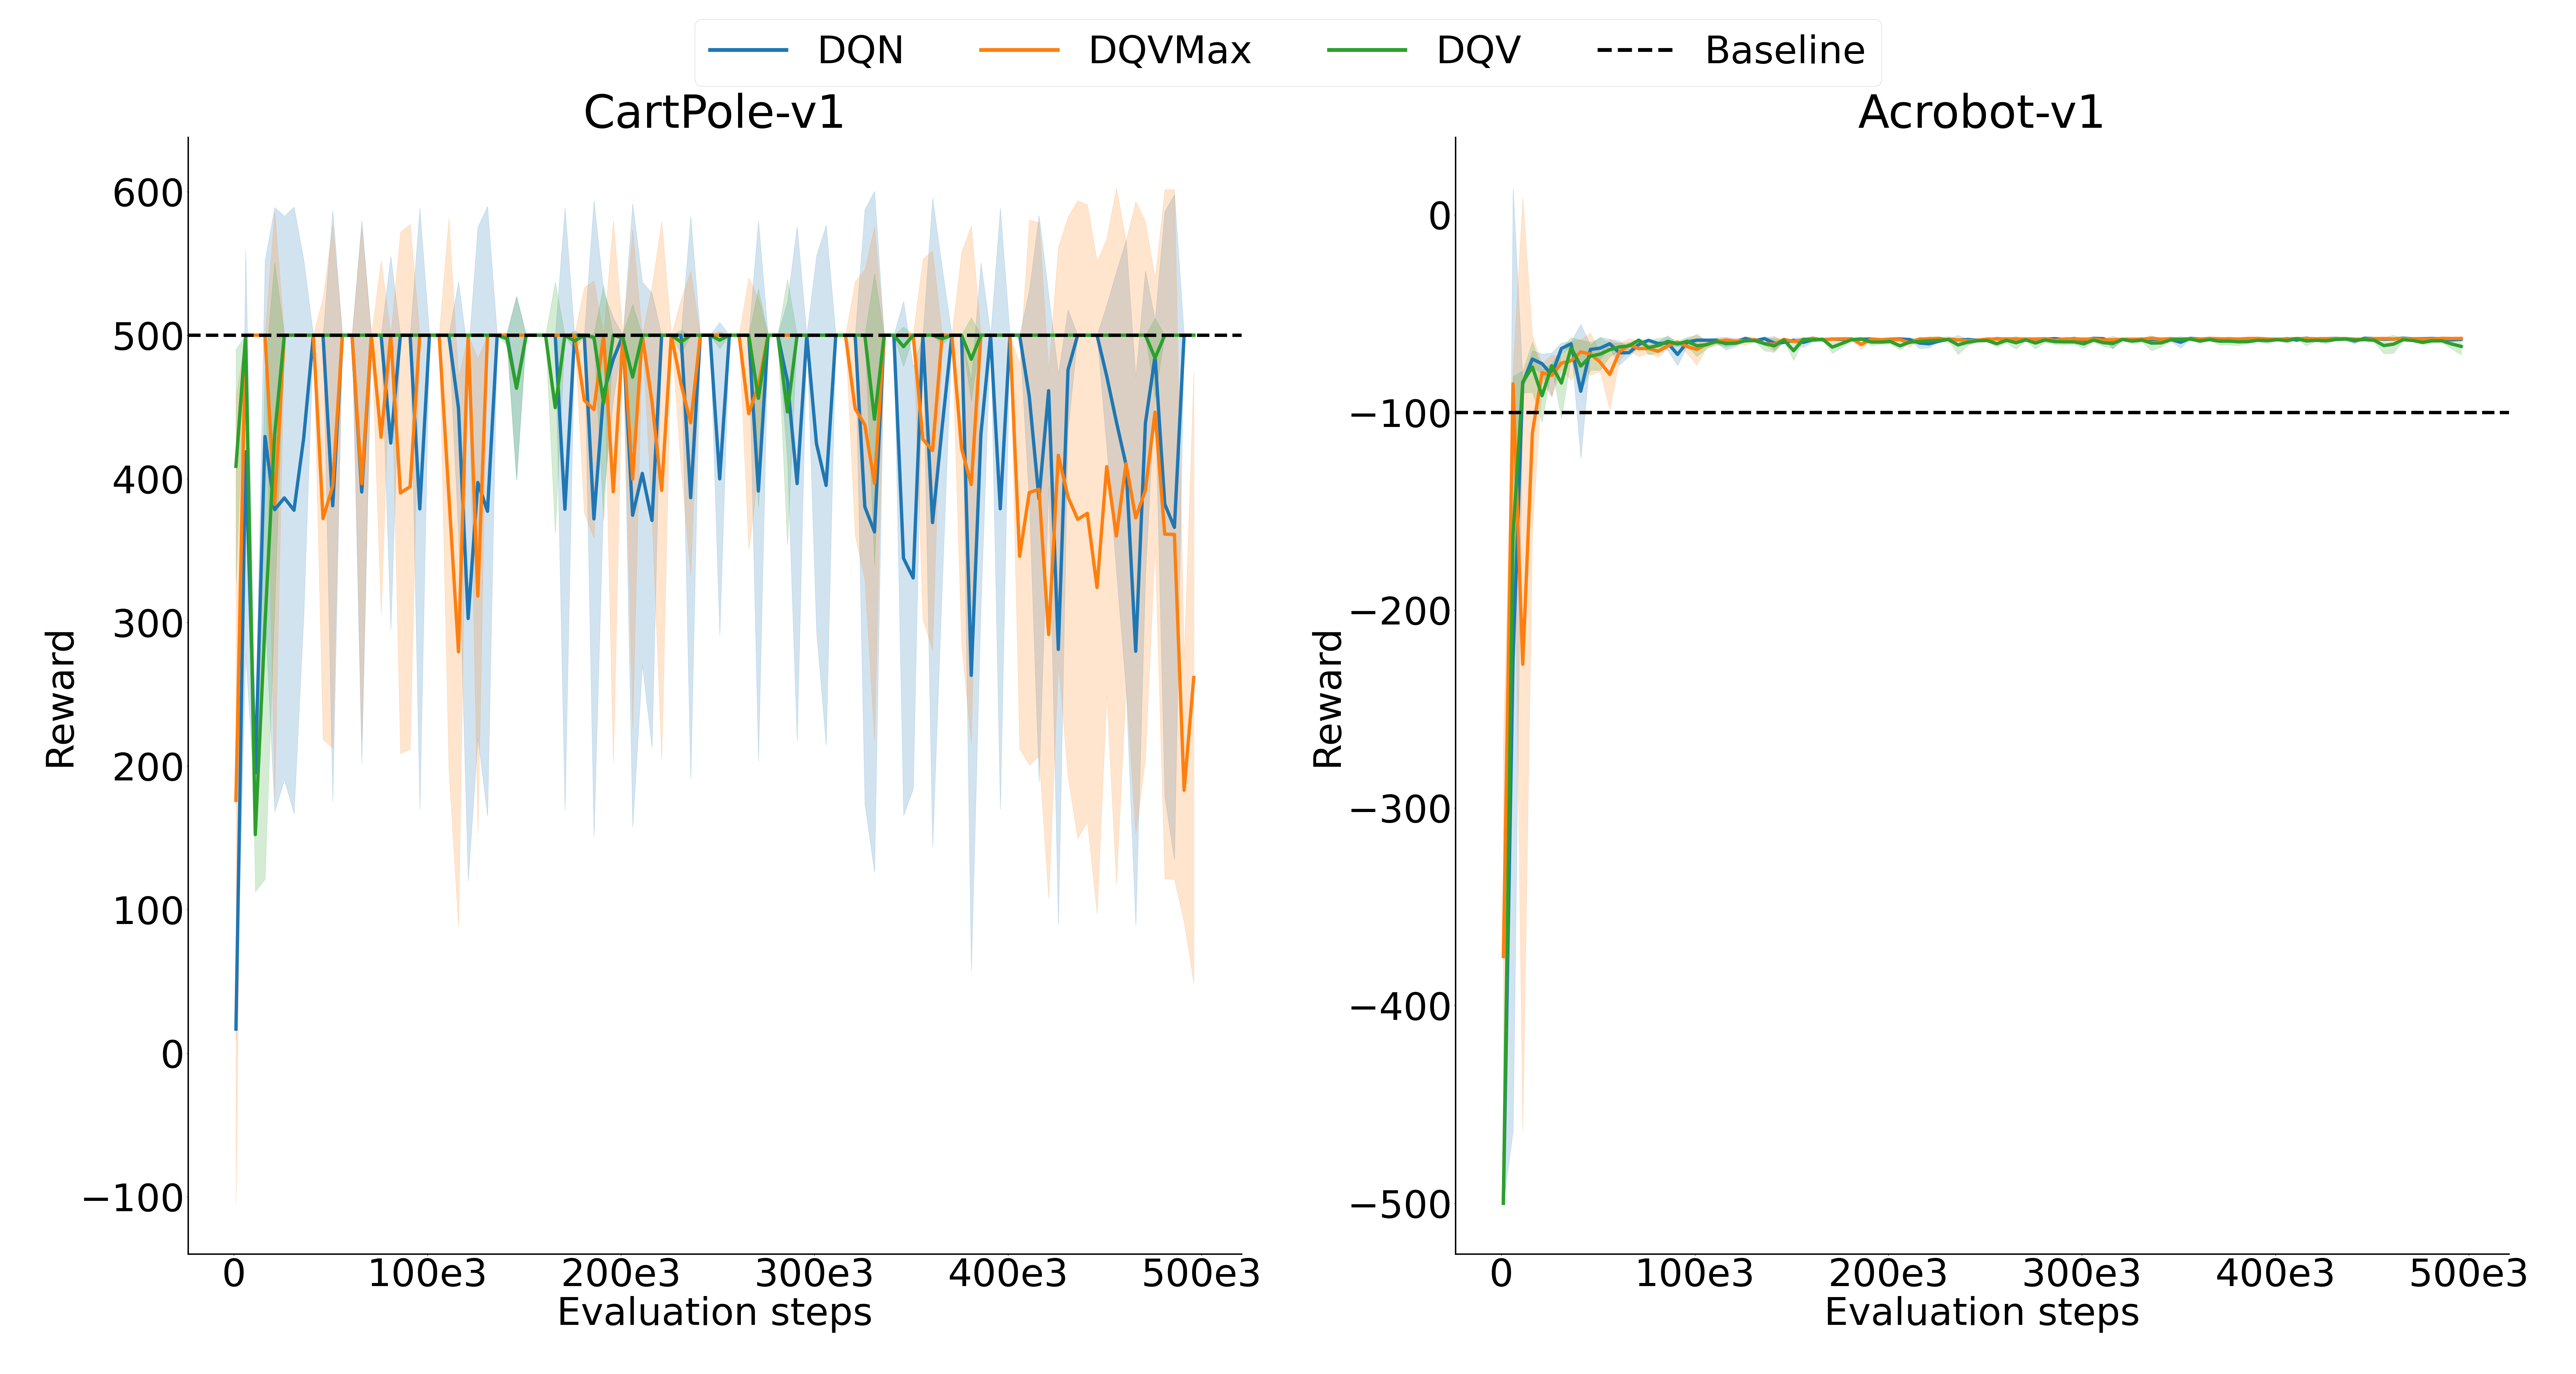
\includegraphics[width=.5\textwidth]{img/dshift_plots_rwd.png}
  \caption{Standard reward}\label{fig:dshift_rwd}
\end{figure}

\begin{figure}[!tbp]
  \centering
  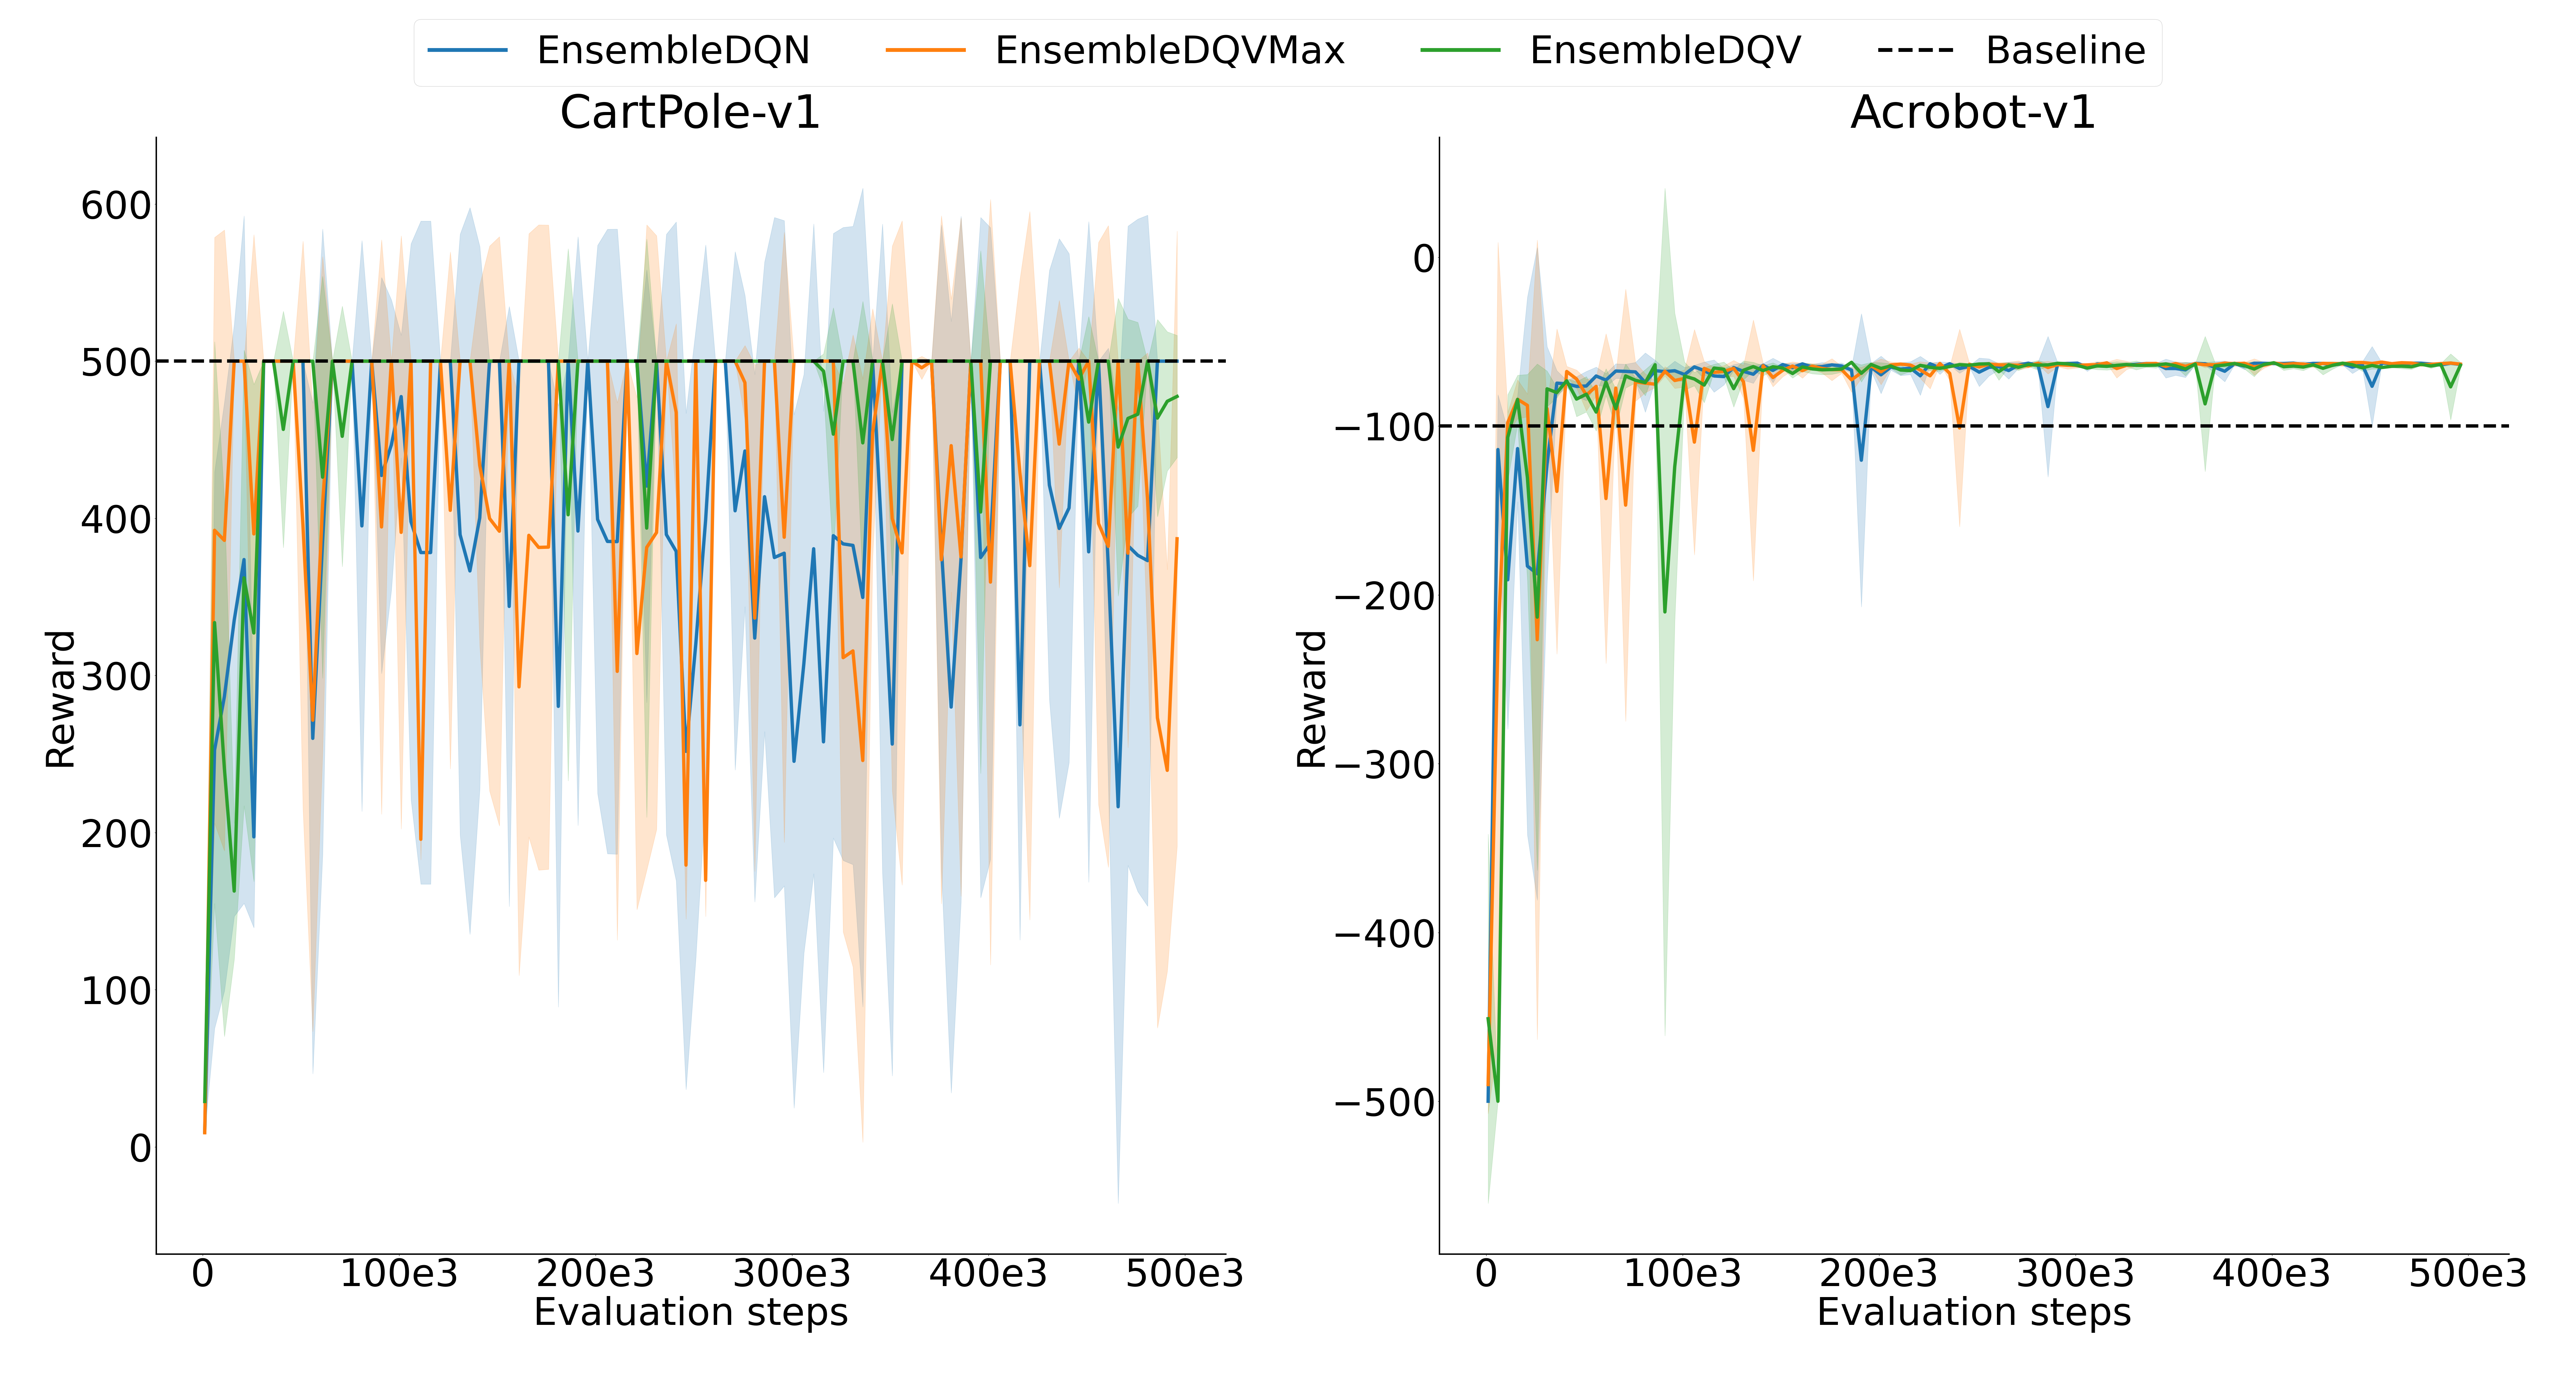
\includegraphics[width=.5\textwidth]{img/dshift_plots_ensembles_rwd.png}
  \caption{Ensemble reward}\label{fig:dshift_ensemble_rwd}
\end{figure}

\begin{figure}[!tbp]
  \centering
  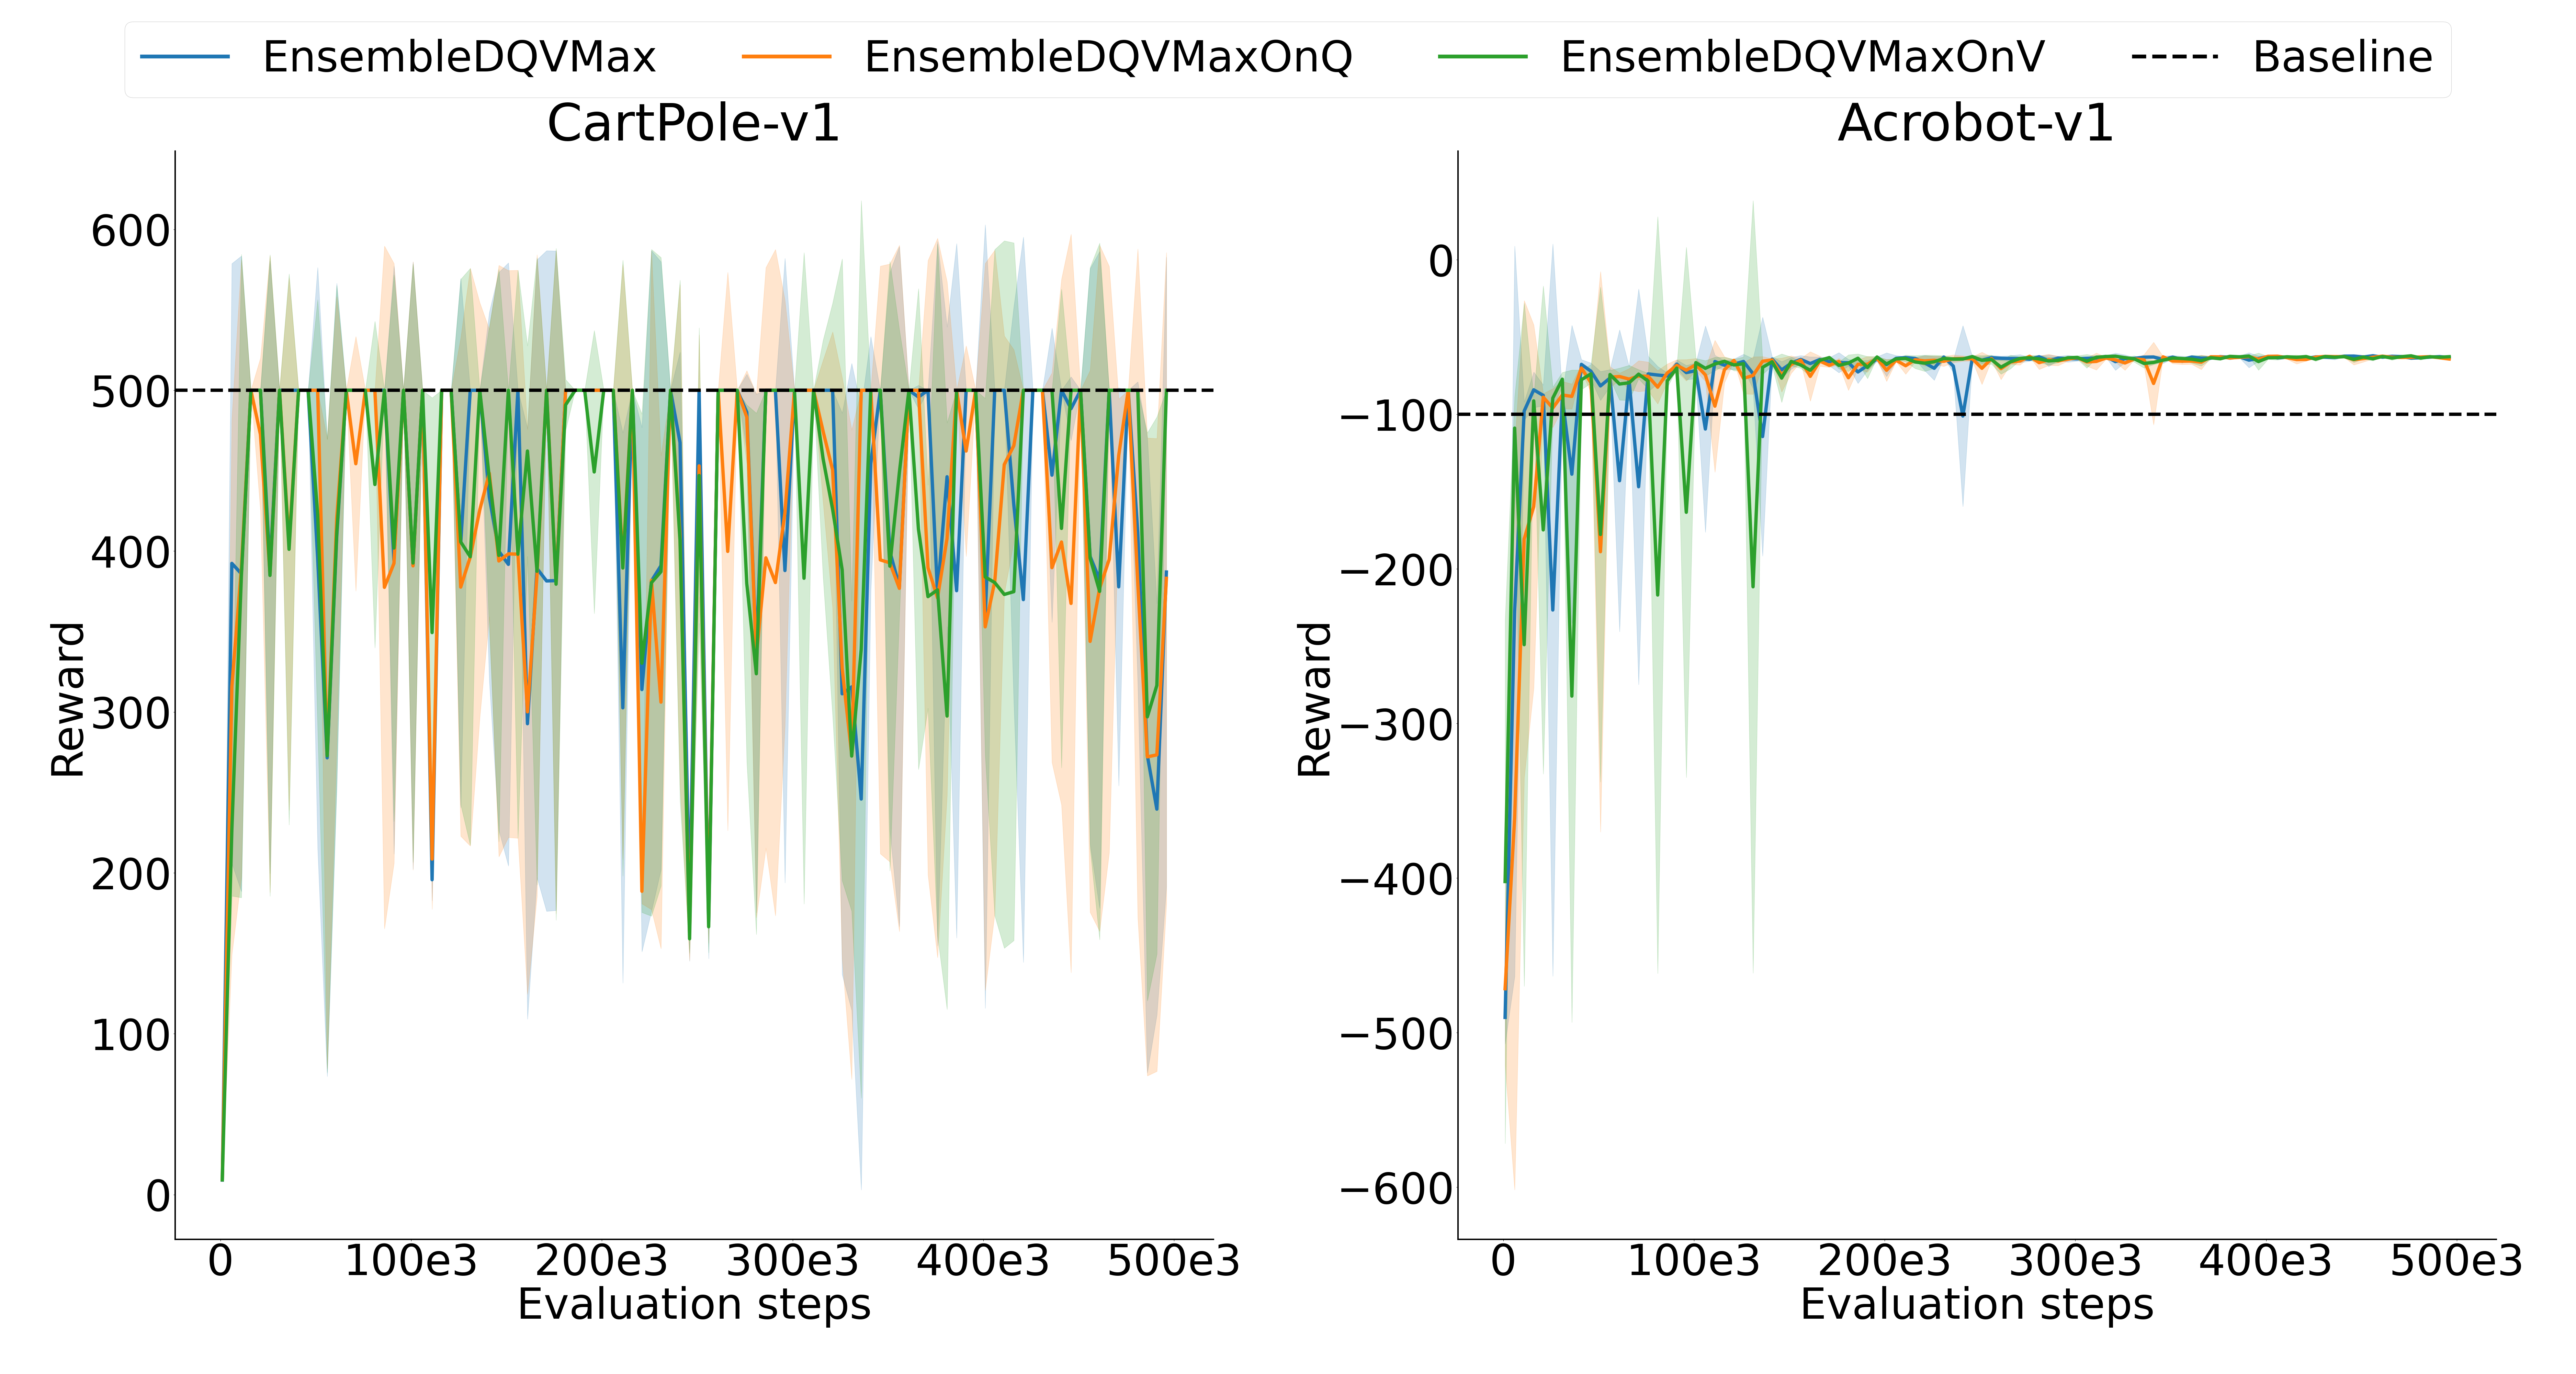
\includegraphics[width=.5\textwidth]{img/dshift_plots_ablation_rwd.png}
  \caption{Ensemble-DQV-Max ablations reward}\label{fig:dshift_rwd_ablation}
\end{figure}

\begin{figure}[!tbp]
  \centering
  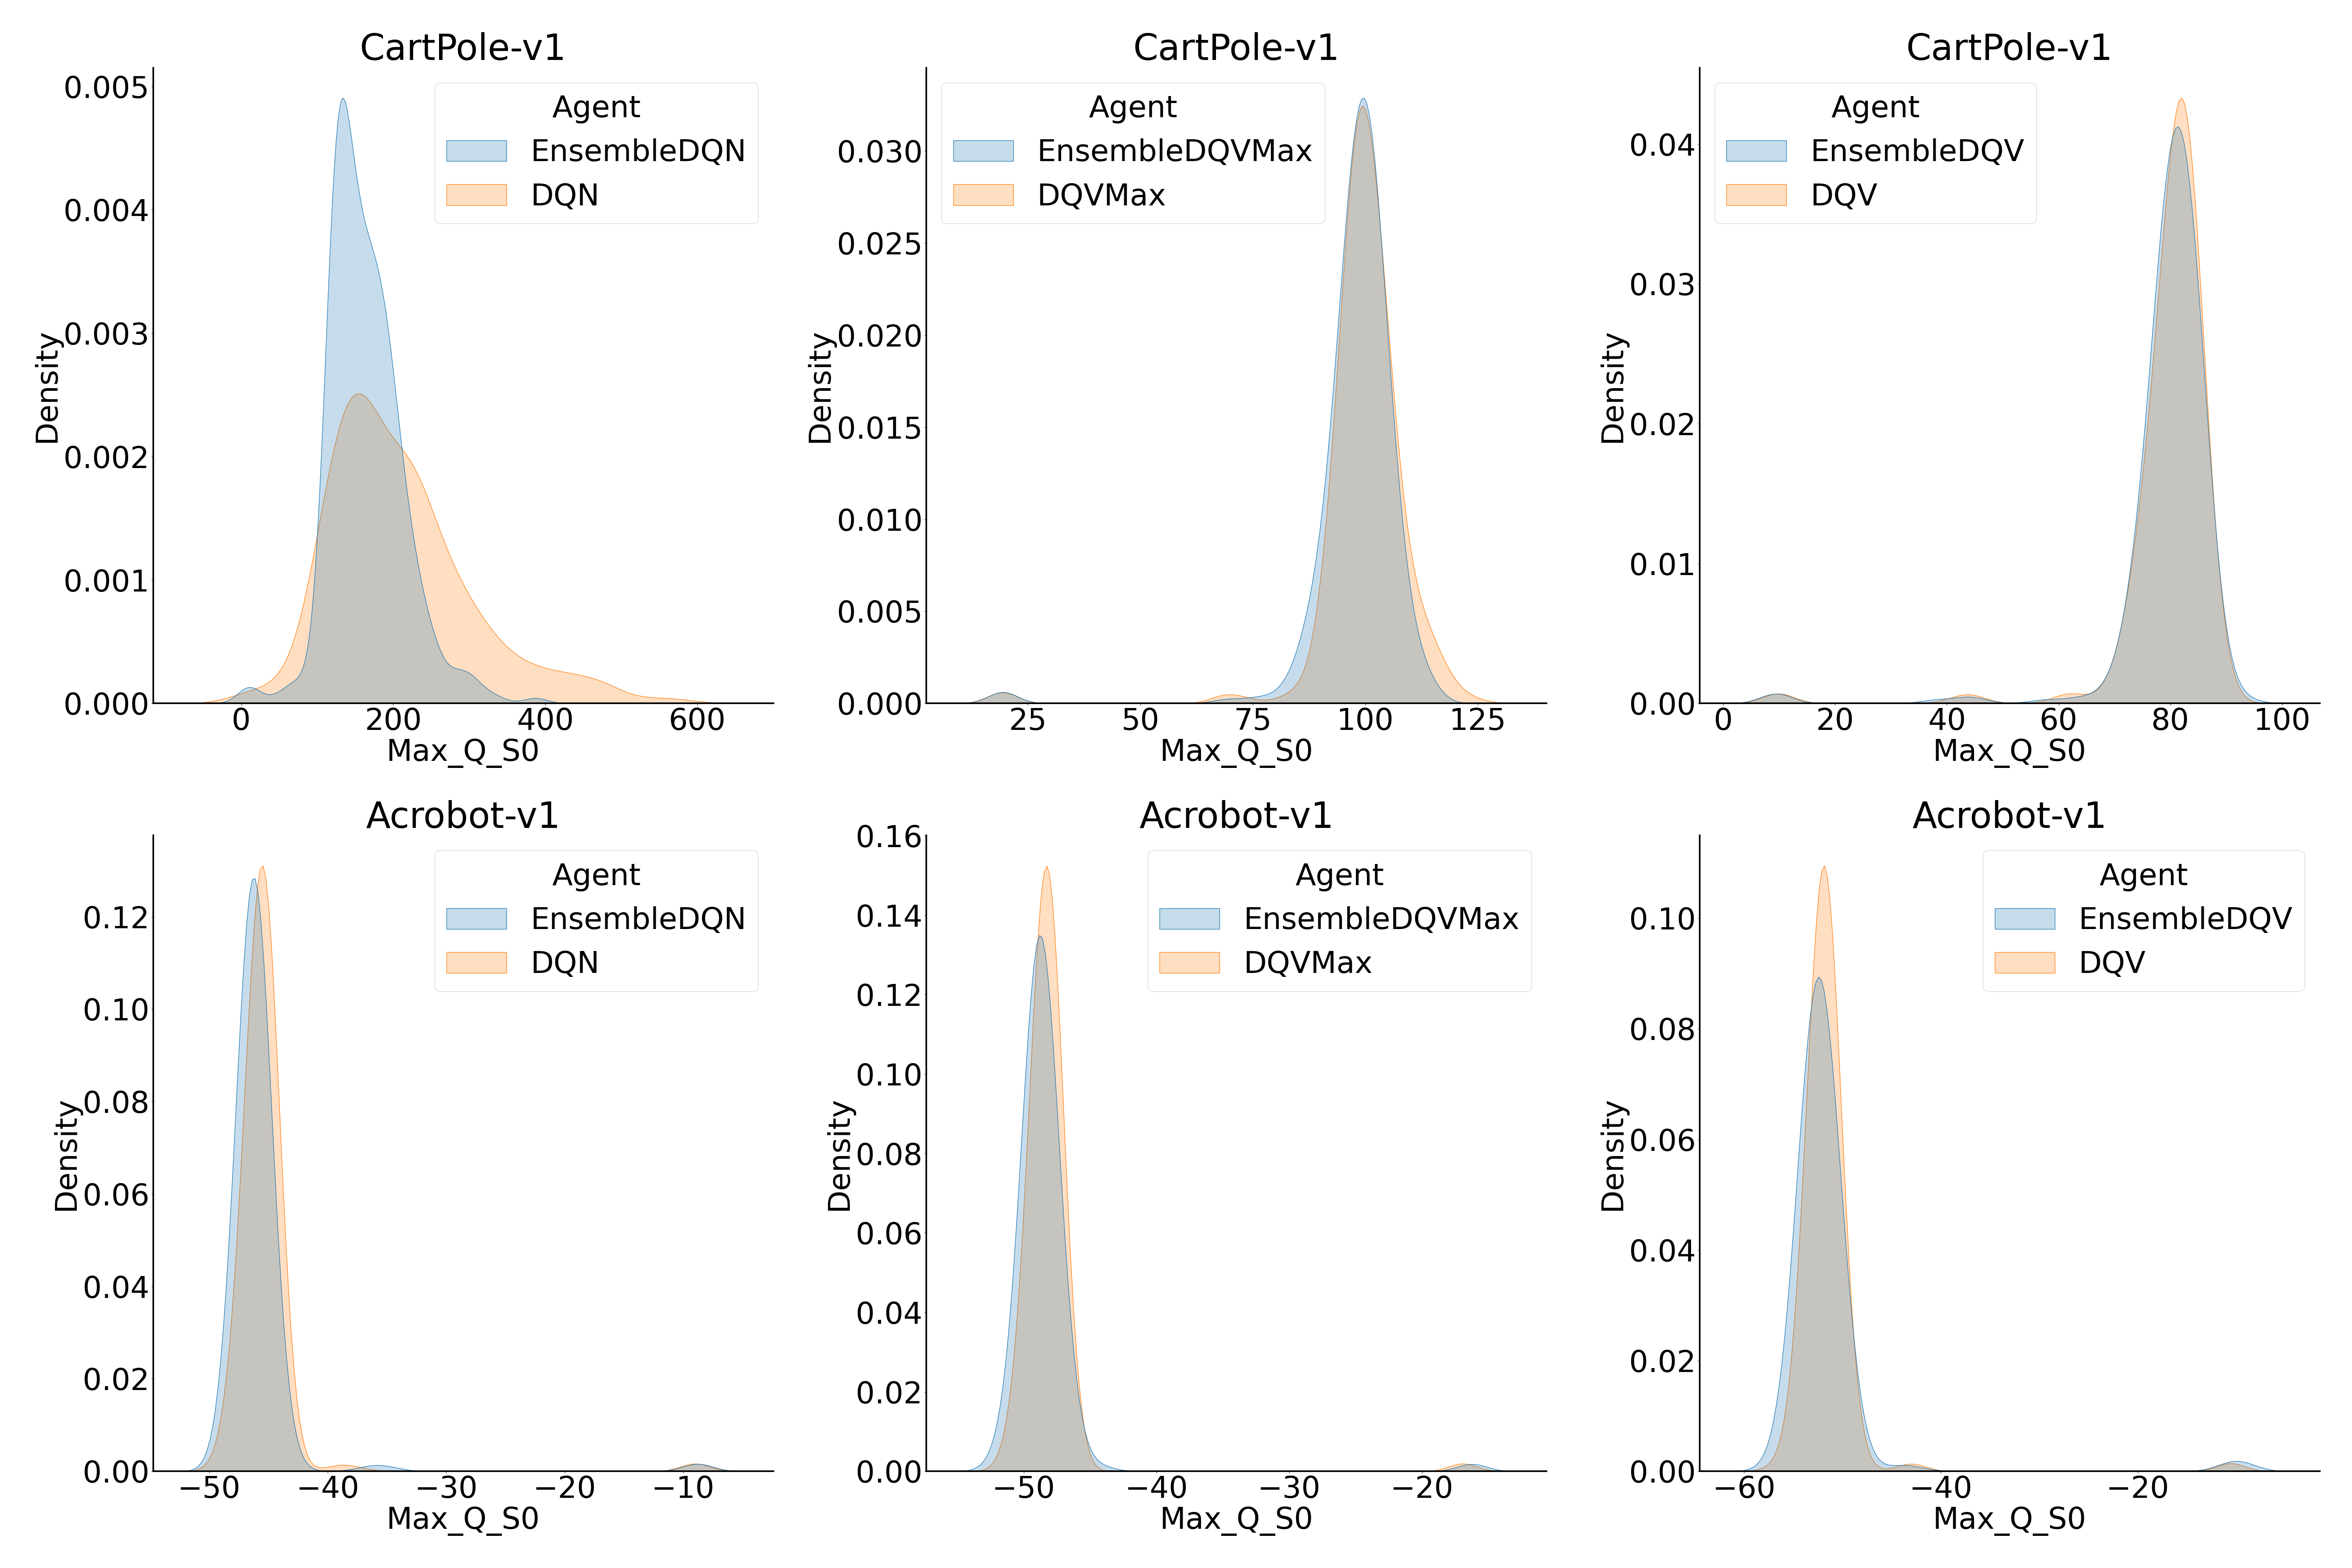
\includegraphics[width=.5\textwidth]{img/all_qv_dist.png}
  \caption{Distribution of Max Q S0 for each agent and its ensemble
    variant}\label{fig:qv_dist}
\end{figure}

\begin{figure}[!tbp]
  \centering
  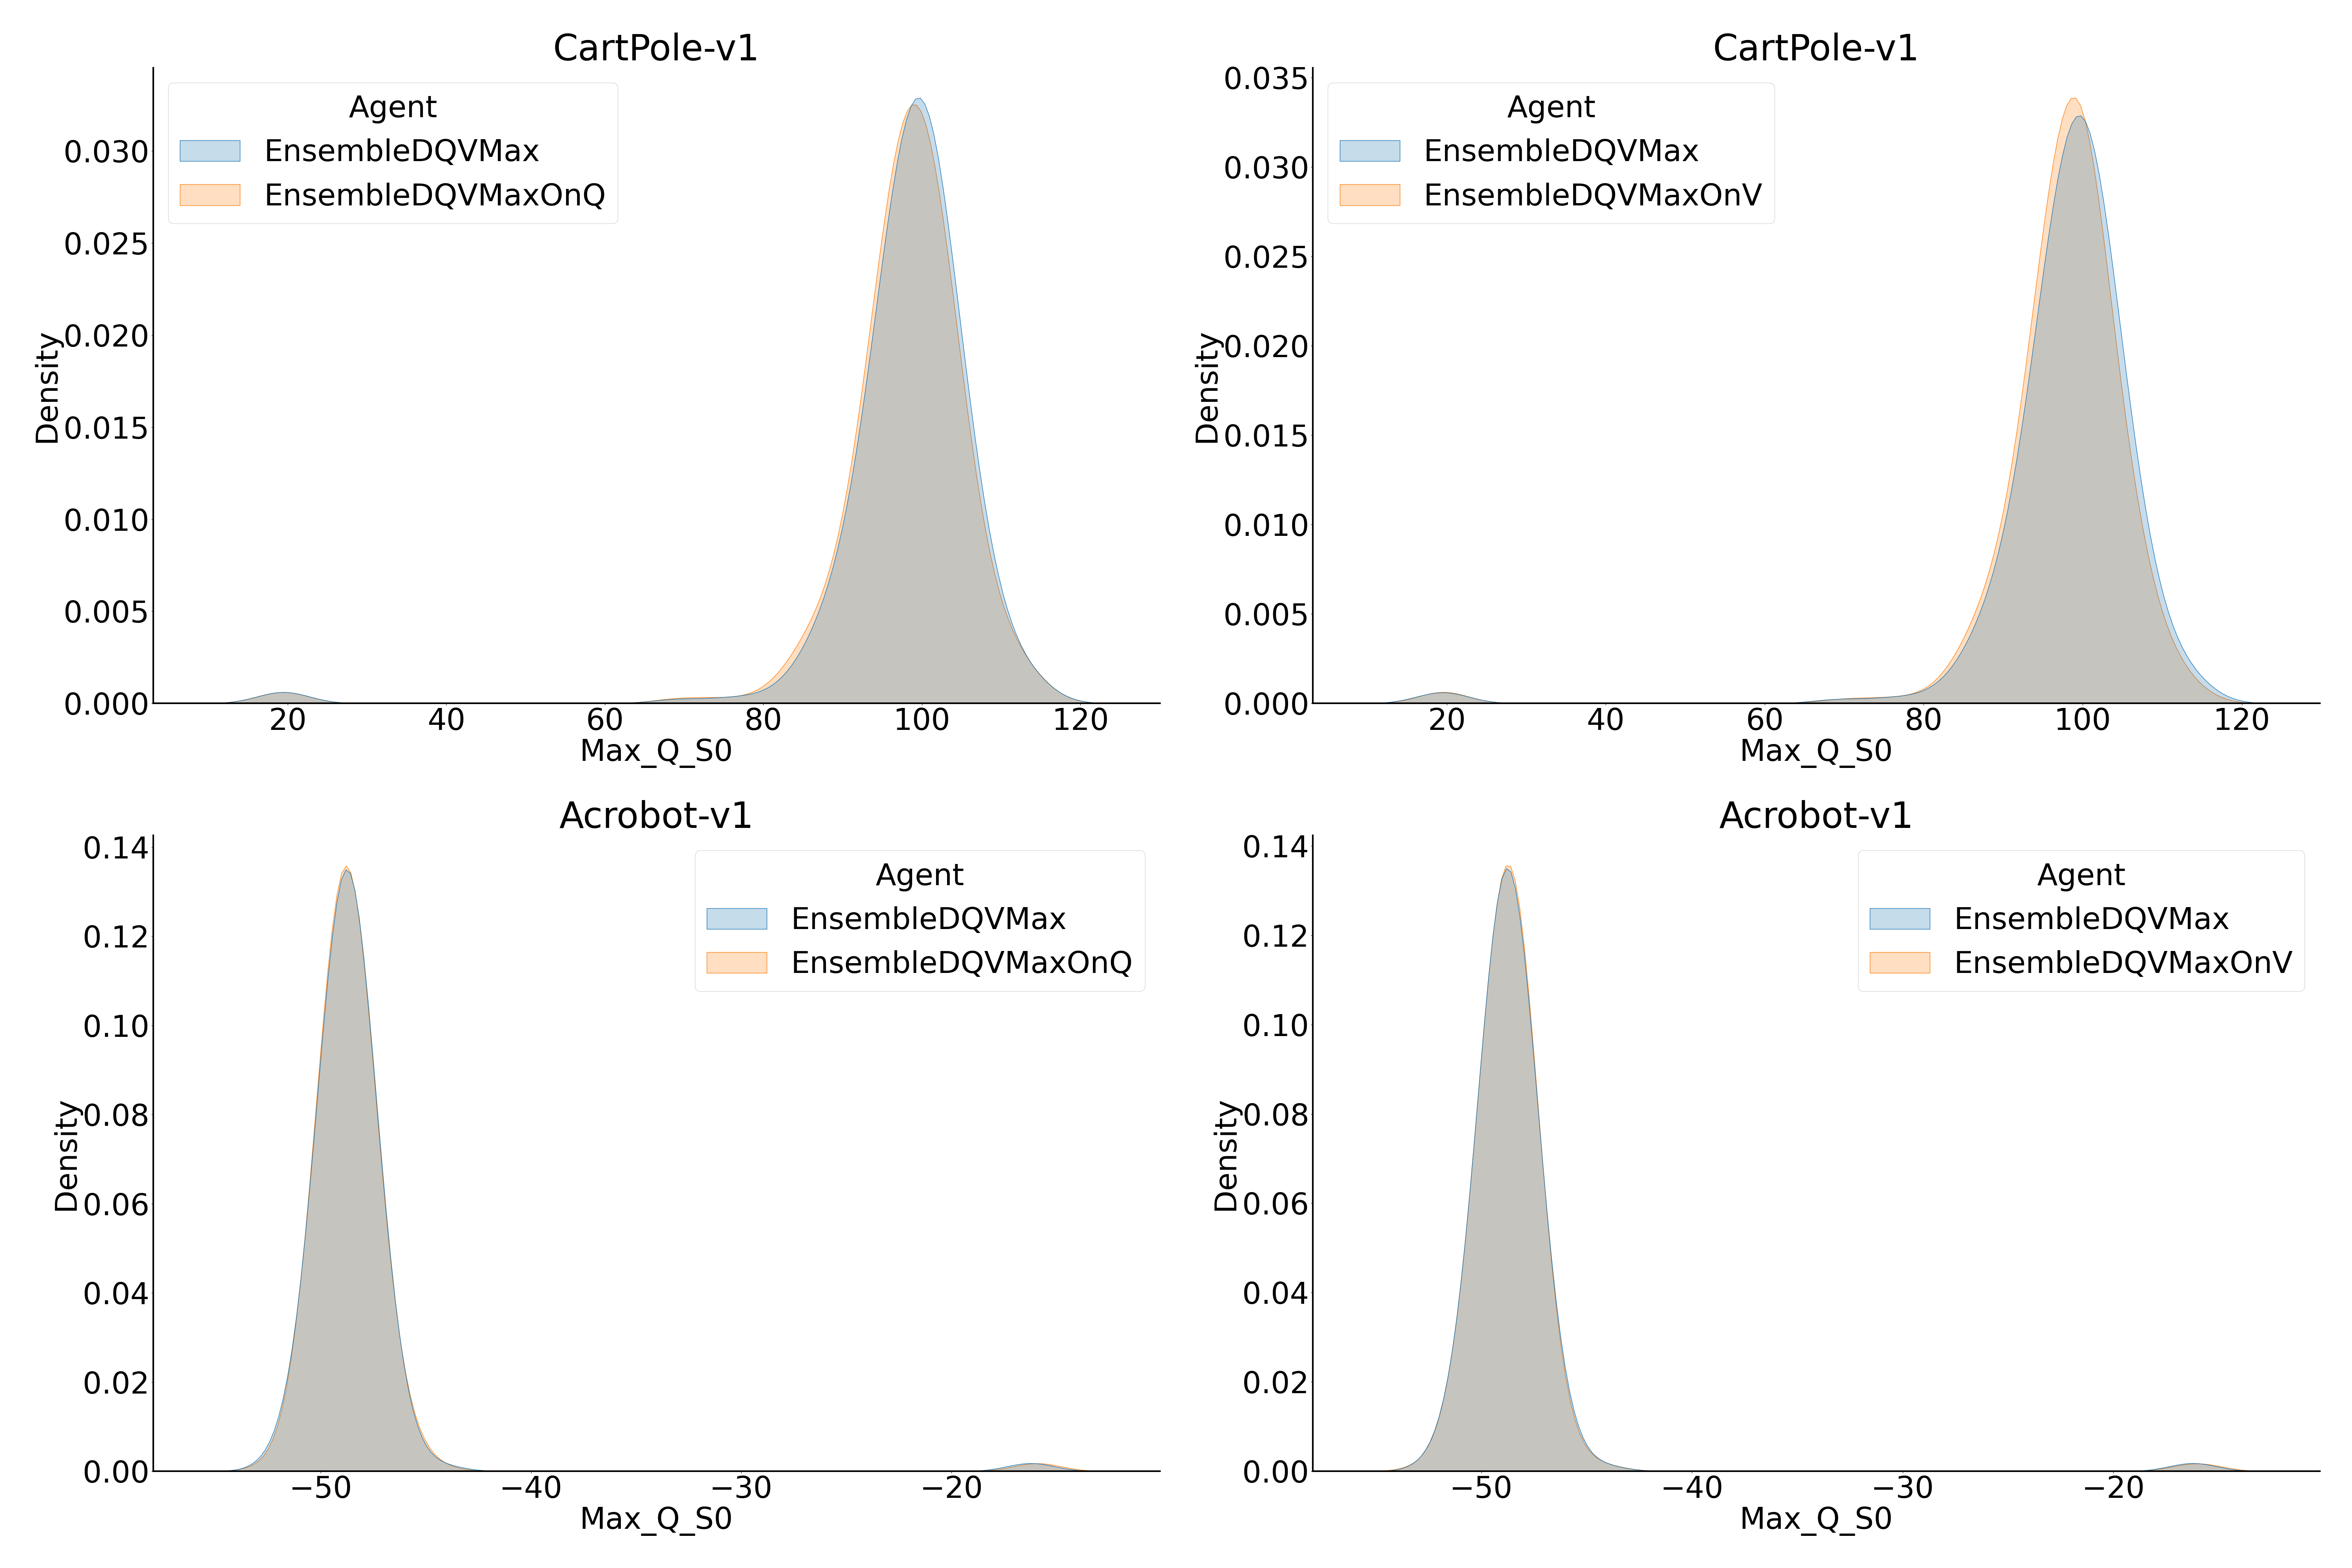
\includegraphics[width=.5\textwidth]{img/dqvmax_abl_qv_dist.png}
  \caption{Distribution of Max Q S0 for Ensemble-DQV-Max and its
    ablations}\label{fig:dqvmax_abl_qv_dist}
\end{figure}

\begin{figure}[!tbp]
  \centering
  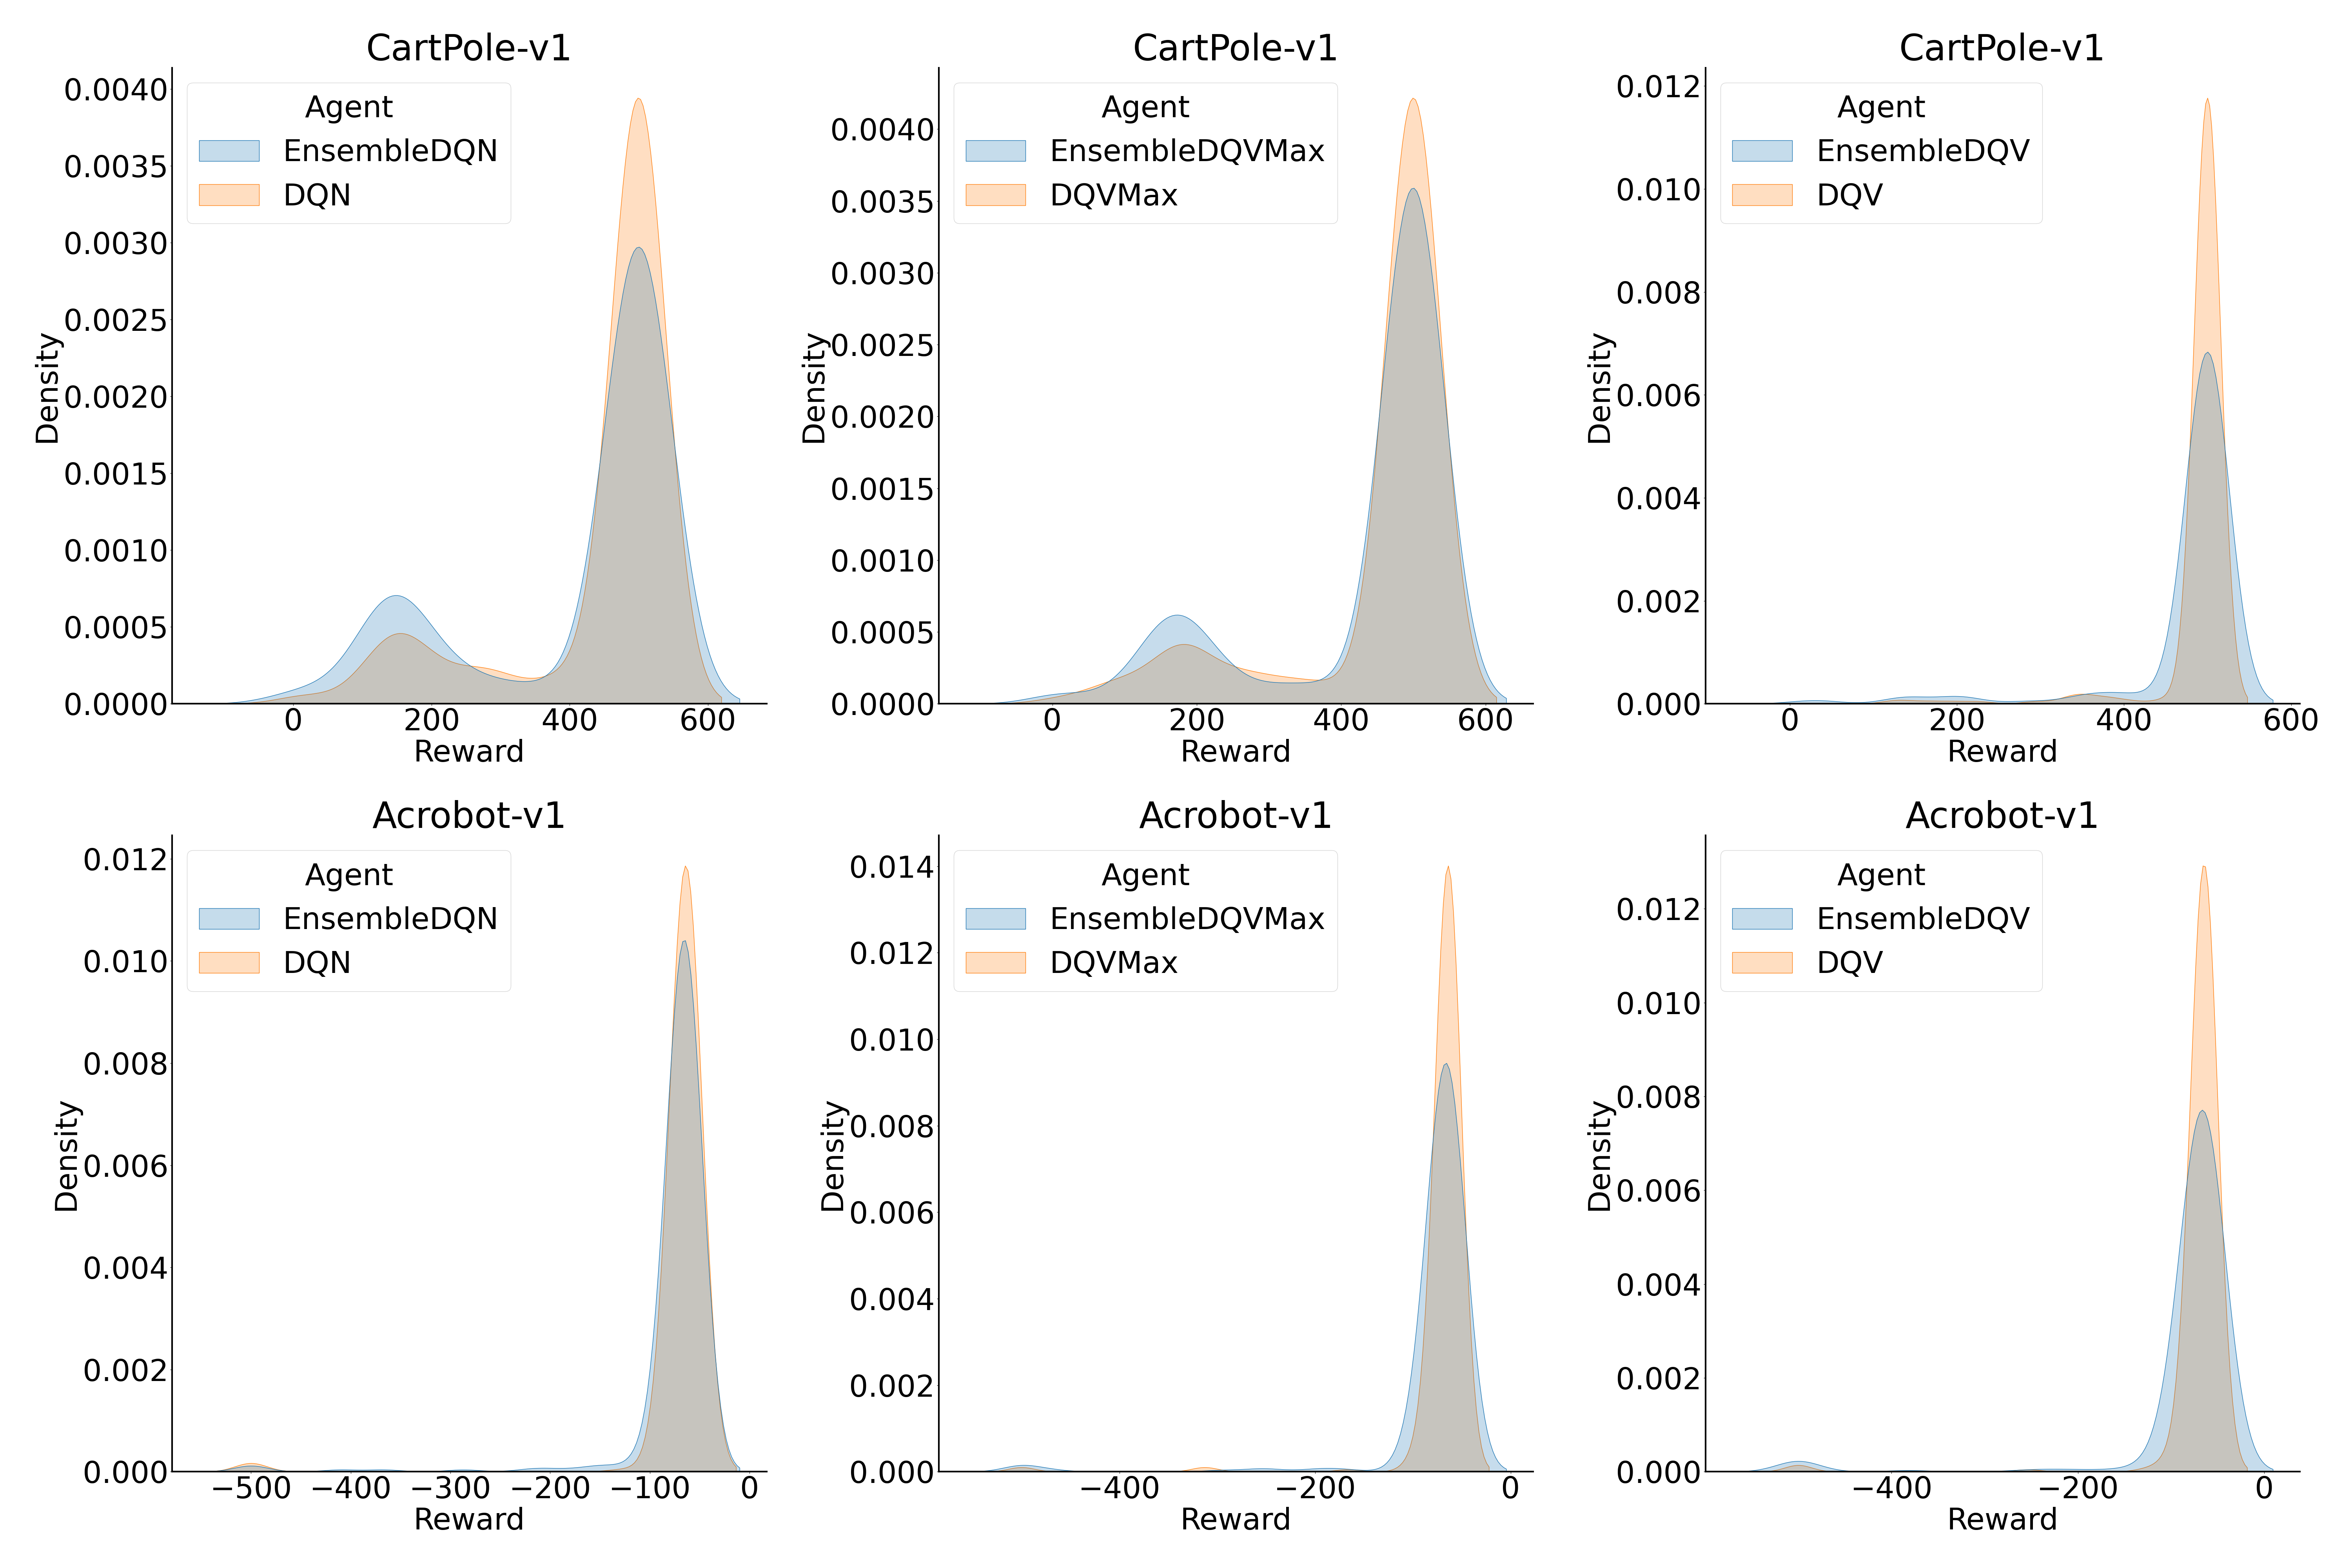
\includegraphics[width=.5\textwidth]{img/all_rwd_dist.png}
  \caption{Distribution of rewards for each agent and its ensemble
    variant}\label{fig:rwd_dist}
\end{figure}

\begin{figure}[!tbp]
  \centering
  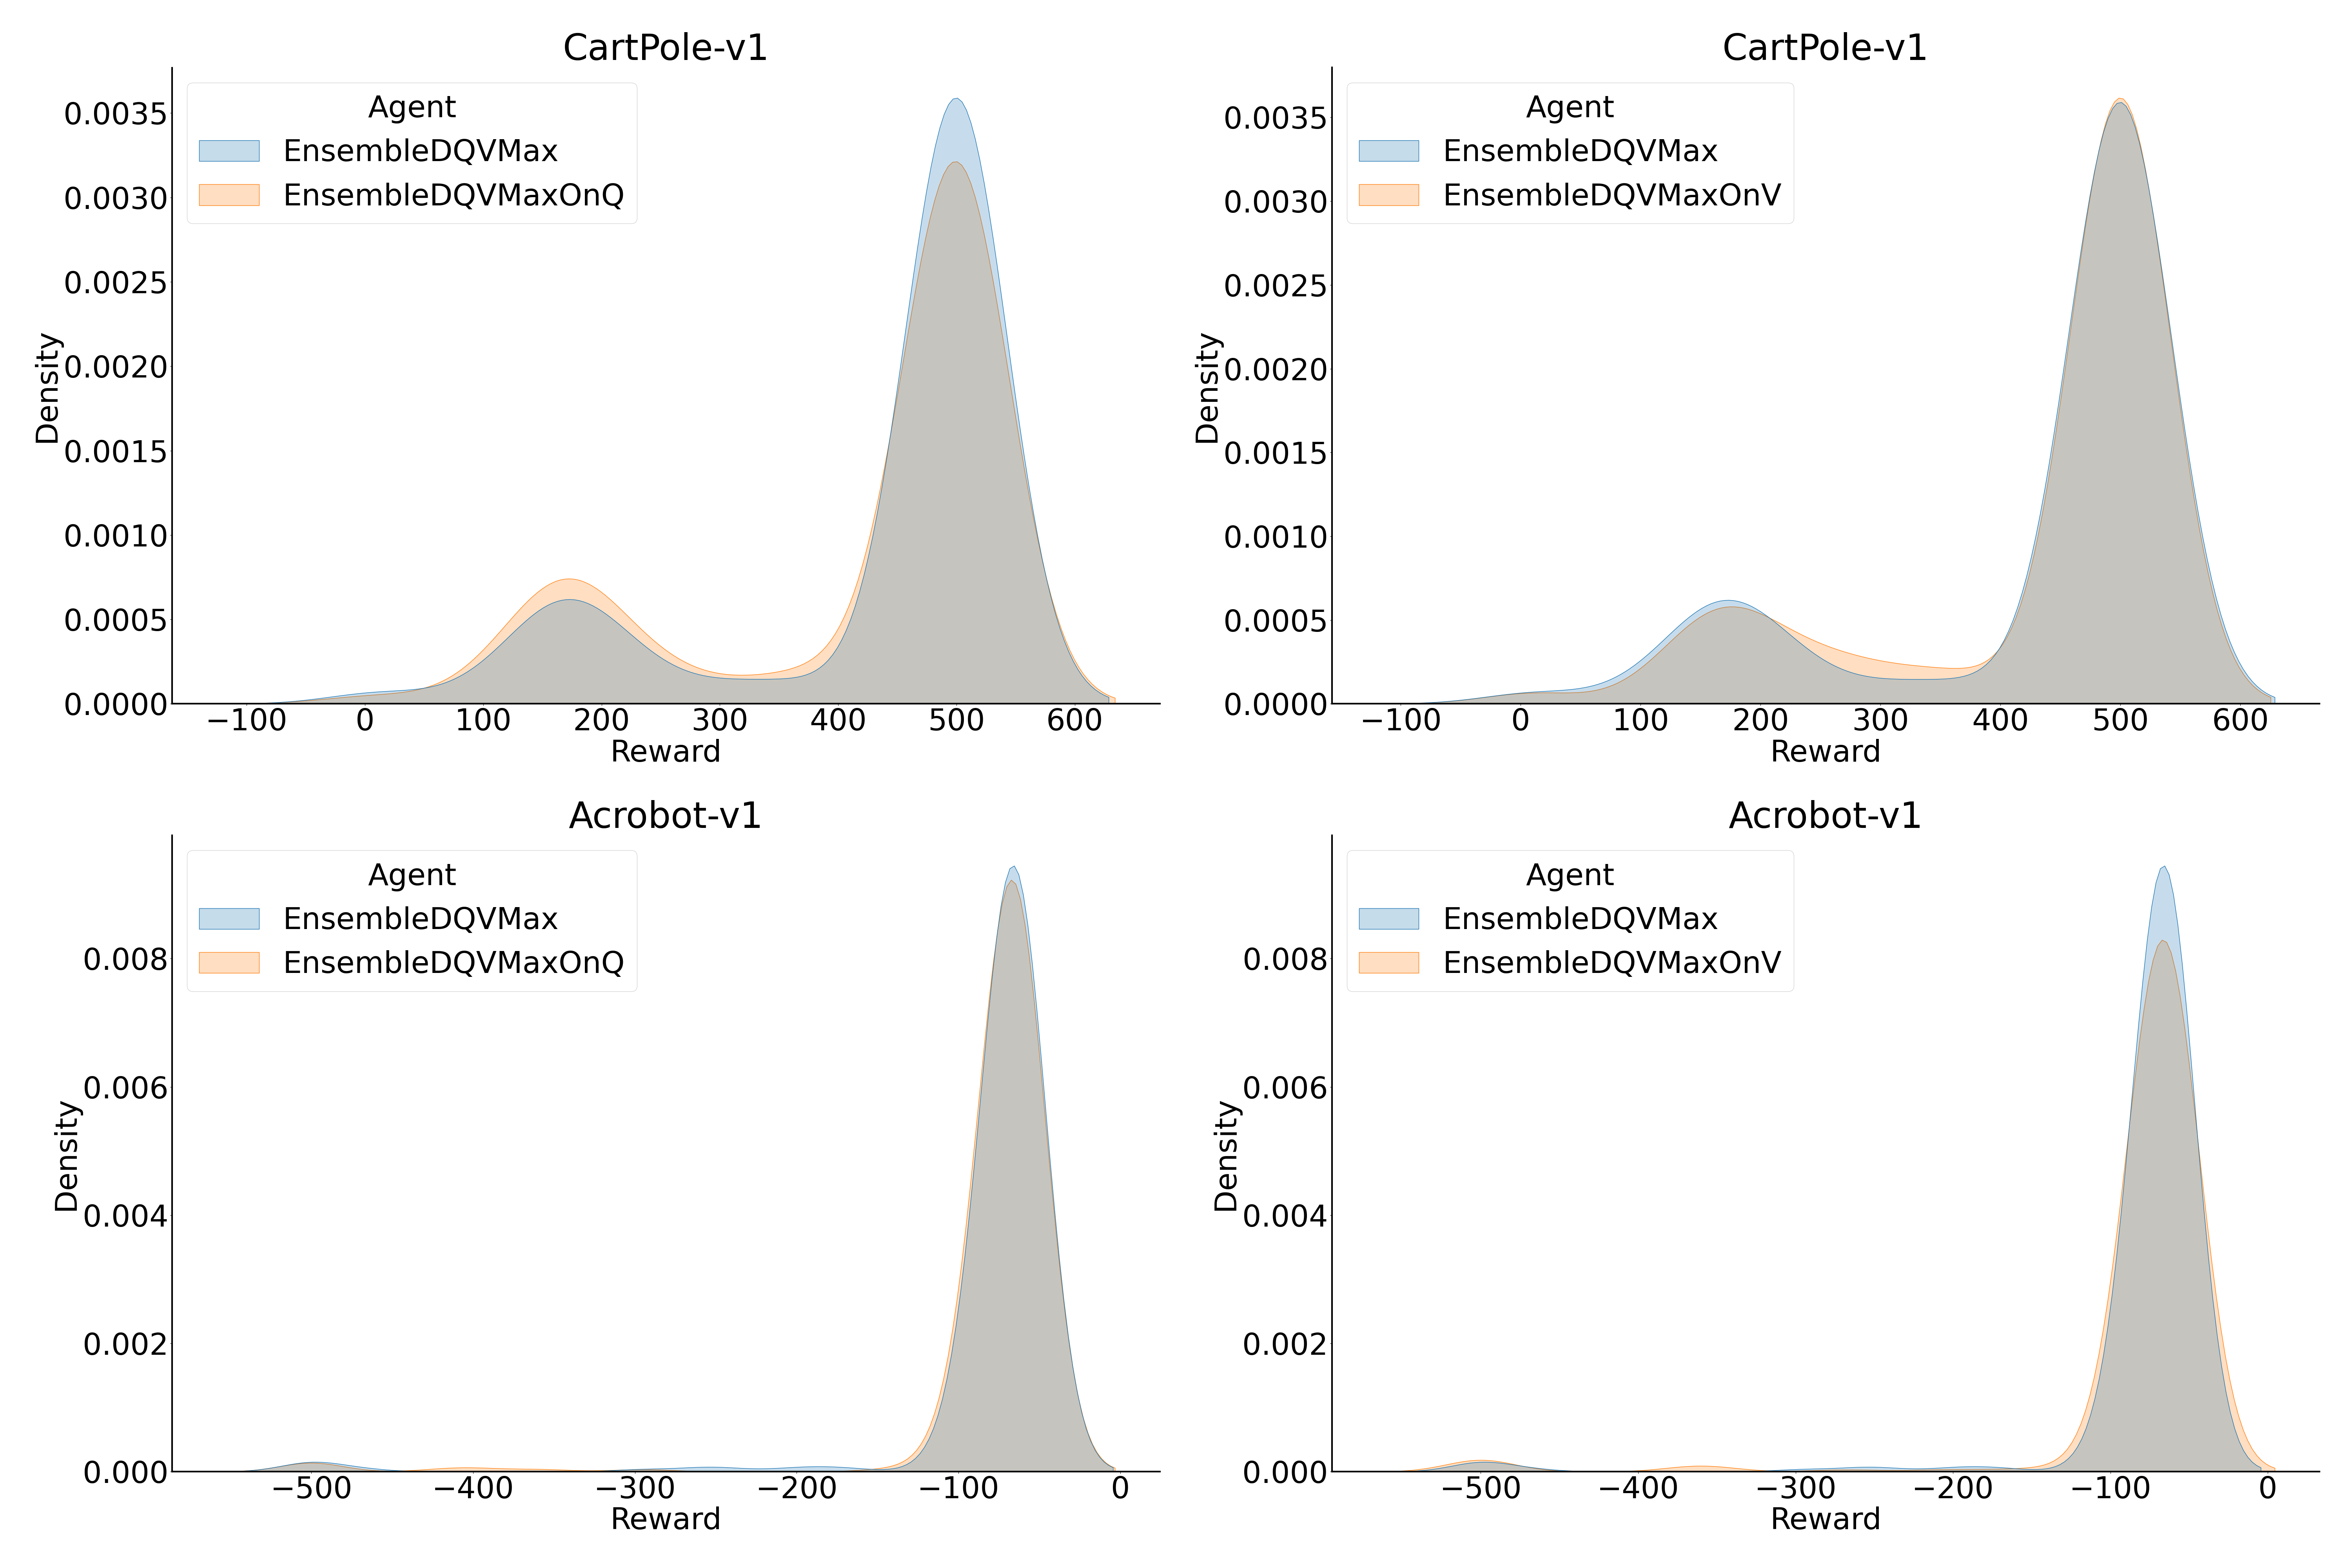
\includegraphics[width=.5\textwidth]{img/dqvmax_abl_rwd_dist.png}
  \caption{Distribution of reward for Ensemble-DQV-Max and its
    ablations}\label{fig:dqvmax_abl_rwd_dist}
\end{figure}
